\documentclass[Royal,times,sageh]{sagej}

\usepackage{moreverb,url,natbib, multirow, tabularx}
\usepackage[colorlinks,bookmarksopen,bookmarksnumbered,citecolor=red,urlcolor=red]{hyperref}



% tightlist command for lists without linebreak
\providecommand{\tightlist}{%
  \setlength{\itemsep}{0pt}\setlength{\parskip}{0pt}}



\usepackage{float}
\usepackage{booktabs}
\usepackage{caption}
\usepackage{longtable}
\usepackage{colortbl}
\usepackage{array}
\usepackage{anyfontsize}
\usepackage{multirow}


\begin{document}


\setcitestyle{aysep={,}}

\title{canaccessR: An open data product for analyzing transportation
accessibility to employment and grocery stores in Canada's largest
metropolitan areas.}

\runninghead{}

\author{João Pedro Figueira Amorim Parga\affilnum{}, Anastasia
Soukhov\affilnum{}, Robert Nutifafa Arku\affilnum{}, Christopher
Higgins\affilnum{}, Antonio Páez\affilnum{}}

\affiliation{}



\begin{abstract}
In this paper, we describe the \{canaccesR\} package, an open data
product (ODP) created in R that contains public transit travel time
estimates to employment locations and grocery stores across Canada's 12
largest metropolitan areas. We calculate travel time matrices (TTM) from
and to each Dissemination Area (DA) within these regions for the years
2019 and 2023. We add value to the urban analytics community by
processing and integrating raw data, and disseminating user-ready data
in the domain of transportation accessibility in Canada. To do so, we
use the \{r5r\} R package, General Transit Feed Specification (GTFS),
OpenStreetMap (OSM), DMTI's Enhanced Points of Interest, and Statistics
Canada Census data. This data package can be used by researchers,
practitioners, and transit agencies to estimate accessibility levels to
these two essential destinations within these urban areas. Moreover,
these estimations can be used as inputs in equity and inequalities
assessments, through the comparisons of within and across accessibility
levels found throughout Canada's largest metropolitan areas.
Consequently, we expect to contribute to informed and data-based
decision making in transportation by disseminating these data. We hope
that these datasets can substantiate future improvements in
policy-making that may lead to greater justice in the country's urban
transportation systems. The package is still in its initial phase and
may undergo expansions in the future by adding TTM's for other
destinations (e.g., schools, healthcare facilities). Finally, as an
ODPs, the \{canaccess\} package allows for open exploration, use, and
contribution by users through its GitHub repository.
\end{abstract}

\keywords{Public transit accessibility; open data products (ODPs); R
data package; travel time matrices.}

\maketitle

\section{Introduction}\label{introduction}

The objective of this paper is to describe the \{canaccesR\} open data
package. Its main contents are a set of public transit travel time
matrices (TTM) estimates to employment and groceries stores from the 12
largest Canadian metropolitan areas in 2019 and 2023, representing
approximately 55\% of the Canadian population. The results are provided
at the Dissemination Areas (DA) \footnote{Dissemination Areas are the
  smallest publicly available spatial unit provided by Statistics Canada
  \citep{governmentofcanadaDictionaryCensusPopulation2021a}.} level,
yielding origin-destination pairs containing associated travel time by
public transit, population, total employment, mode share, and other
relevant census variables and spatial shape boundaries for each
metropolitan area. This data package was created by leveraging expertise
in data science, R programming, and transportation analysis. It includes
.Rmd notebooks written for computing travel time matrices for large sets
of origin-destination pairs using the \{r5r\} R package
\citep{pereiraR5rRapidRealistic2021}. Overall, \{canaccesR\} offers 52
complementary objects ready for temporal and spatial analysis. The
package is an analysis-read product based on a fusion of data sources,
including public transit schedules (GTFS files), road and transit
networks, census data, and filtered business location data.

TTMs are a core piece of information required for estimating spatial
interaction. Accessibility -the \emph{potential} spatial interaction
offered by the transportation system to reach destinations
\citep{paezMeasuringAccessibilityPositive2012}- is an example of a
measure that requires TTMs. Recent efforts following an open-source and
transparent philosophy have been made to disseminate useful data and
information on transportation in the Canadian context
\citep{soukhovTTS2016RDataSet2023}. However, despite these initiatives,
pre-processed and available data that allow for the ease estimation of
accessibility indicators are still scarce. Within this context, we
expect to help filling this gap by the processing raw into user-ready
data and making them publicly available to advance knowledge on the
field. Our main contribution is to provide analysis-ready data for
Canada's largest cities on the topic of transportation accessibility,
thus making urban analytics in the country more accessible and
contributing to future research and data-based decision making.

The package's main audiences are Canadian researchers in urban planning
and transportation and transportation system agencies. We anticipate
three primary uses for the open data product (ODP) described in this
paper. First, the datasets allow for static assessment of the level of
public transit accessibility across the country's largest cities before
and after the COVID-19 pandemic. In other words, \{canaccesR\} makes it
easier for those interested in comparing cities regarding their level of
public transit accessibility to essential destinations (such as
employment centers and groceries stores) to do so. Second, the temporal
and spatial characters of the datasets made available here allow
researchers to evaluate accessibility changes through time and across
space within the largest Canadian urban areas. Third, as is now common
practice in transportation accessibility research, used as inputs, these
estimates can substantiate broader investigations on transportation
justice and equity
\citep{higginsChangesAccessibilityEmergency2021, humbertoHowTranslateJustice2023, pereiraGeographicAccessCOVID192021}.
For example, the TTM estimates allow for evaluating the evolution of
public transit's accessibility by income or spatial distribution across
all Dissemination Areas (DA's) of each of the 12 cities in the sample
\citep{pargaDemocraticAccessOur2024}. In other words, the package's
contents can be used from straightforward assessments of accessibility
in Canadian urban areas to more theoretically and morally complex
evaluations of justice in the country's urban transportation system.

Besides this introduction, we organize this paper as follows. The next
section contains a description of the data sources we used to construct
the data package. Then, we recount the data processing necessary to
create the package. Next, we go through the main contents of the data
package, i.e., the travel time matrices estimated through our analysis.
We present some basic descriptive statistics of these datasets, and
elucidate how one can use them in accessibility analysis. Finally, we
conclude by explaining how we expect \{canaccesR\} to contribute to the
urban analytics and science community.

\section{Data and methods}\label{data-and-methods}

\subsection{Raw data sources}\label{raw-data-sources}

The locations included in the data package comprise the 12 largest
(population-wise) Census metropolitan areas (CMA's) based on the 2016
Canadian Census \citep{governmentofcanada2016CensusPopulation2016}
\footnote{We included Oshawa as part of the Greater Toronto Area (GTA)
  because of its proximity. Similarly, we included Abbotsford-Mission as
  part of the Vancouver metropolitan area due to its proximity to a
  transit station on the region's West Coast Express commuter rail line.}.These
locations are the surrunding Toronto, Montreal, Vancouver,
Ottawa-Gatineau, Calgary, Edmonton, Quebec City, Winnipeg, Hamilton,
Kitchener-Cambridge-Waterloo, London, and Halifax areas. We used four
main data sources to construct the \{canaccesR\} data package: General
Transit Feed Specification (GTFS), OpenStreetMap (OSM), DMTI's Enhanced
Points of Interest, and Statistics Canada Census data.

We manually collected and processed the GTFS files from all transit
agencies within the selected CMA's to use their information on the
public transit schedule in 2019 and 2023. The OpenStreetMap data for the
selected areas were collected through the \{osmextract\} package
\citep{gilardiOsmextractDownloadImport2025}. We used OSM data from 2019
and 2023, which provided information on the areas' transit network in
two points in time. We collected data from the 2016 Canadian Census
using the \{cancensus\} package
\citep{vonbergmannCancensusPackageAccess2022} and used its information
on the spatial distribution of the population and the number of
workplace locations (employment) across the CMA's
\citep{governmentofcanada2016CensusPopulation2016}. Finally, we gathered
and cleaned the 2023 DMTI's Enhanced Points of Interest dataset to
obtain the location of the groceries stores within every urban area
selected \citep{dmtispatialincEnhancedPointsInterest2015}. We filtered
the locations within the DMTI dataset using the grocery stores code from
the North American Industry Classification System (NAICS) and the
Standard Industrial Classification (SIC). \{\textbf{THE CODE FOR THIS
ESTIMATIONS AND THE TRAVEL TIME MATRICES IS ON THE
transit\_death\_spiral github repo. 1) SHOULD WE CITE IT? 2) IS THAT A
PROBLEM?}\}

\subsection{Methods: travel time matrices
processing}\label{methods-travel-time-matrices-processing}

Using the \{r5r\} R package, we estimated public transit travel times
for two destination types, grocery stores and jobs. For each amenity
type, we chose a likely travel time and day of the week. We set a 15
minutes time window and the maximum trip duration to 120 minutes. The
estimated times are the median of the 15 minute time window. For
groceries stores, we set the departure date to a weekend afternoon and
the departure time to between 12:00 PM to 12:15 PM on April 20, 2019 and
April 22, 2023. For employment, we ran the analysis on a typical weekday
morning rush-hour commute, more specifically 8:00 to 8:15 AM departure
on Tuesday, April 16, 2019 and Tuesday, April 18, 2023 \footnote{The one
  exception is Quebec City, where the routing for 2019 occurs on a
  Saturday and Tuesday in June (instead of April) due to the GTFS data
  unavailability.}. In both cases, we assumed that walking was the mode
of travel from origin to transit stop and from transit stop to
destination. We aggregated all the resulting travel time matrices at the
Dissemination Area (DA) level, which comprise the fundamental unit of
analysis in data package.

\section{\{canaccessR\}'s contents}\label{canaccessrs-contents}

\begin{verbatim}
 [1] "census_data_cma_cal"   "census_data_cma_edm"   "census_data_cma_ggh"  
 [4] "census_data_cma_hal"   "census_data_cma_ldn"   "census_data_cma_mtl"  
 [7] "census_data_cma_ott"   "census_data_cma_que"   "census_data_cma_van"  
[10] "census_data_cma_win"   "census_data_da_cal"    "census_data_da_edm"   
[13] "census_data_da_ggh"    "census_data_da_hal"    "census_data_da_ldn"   
[16] "census_data_da_mtl"    "census_data_da_ott"    "census_data_da_que"   
[19] "census_data_da_van"    "census_data_da_win"    "population_statistics"
[22] "region_background_cal" "region_background_edm" "region_background_ggh"
[25] "region_background_hal" "region_background_ldn" "region_background_mtl"
[28] "region_background_ott" "region_background_que" "region_background_van"
[31] "region_background_win" "transit_statistics"    "travel_matrix_emp_cal"
[34] "travel_matrix_emp_edm" "travel_matrix_emp_ggh" "travel_matrix_emp_hal"
[37] "travel_matrix_emp_ldn" "travel_matrix_emp_mtl" "travel_matrix_emp_ott"
[40] "travel_matrix_emp_que" "travel_matrix_emp_van" "travel_matrix_emp_win"
[43] "travel_matrix_grc_cal" "travel_matrix_grc_edm" "travel_matrix_grc_ggh"
[46] "travel_matrix_grc_hal" "travel_matrix_grc_ldn" "travel_matrix_grc_mtl"
[49] "travel_matrix_grc_ott" "travel_matrix_grc_que" "travel_matrix_grc_van"
[52] "travel_matrix_grc_win"
\end{verbatim}

\begin{verbatim}
 [1] 11 12 13 14 15 16 17 18 19 20
\end{verbatim}

Specifically, the package contains the following contents: 10 data.frame
objects containing the calculated public travel times from DA centroids
to grocery stores and another 10 for DA centroids to DA centroids.
Notably, the \{travel\_matrix\_grc\_ggh\} data.frame, is named after the
acronym for the Greater Golden Horseshoe area, which includes the CMA
regions of Toronto, Hamilton, and Kitchener-Cambridge-Waterloo. Hence,
the 20 travel time data.frames represent public transit travel times for
all 12 CMAs across two sets of destinations. Next, 10 sf objects
represent census data for each DA, including dwelling counts, population
by age bracket, single-parent-headed households, low-income prevalence,
official language knowledge, housing- quality, ownership and
affordability variables, visible minority, newcomer- and immigration-
related variables, educational attainment, and commuting mode shares.
Furthermore, 10 and 10 sf objects represent the CMA areas' boundaries
and backgrounds for plotting the data spatially, respectively. Finally,
2 data.frames contain aggregated population and transit statistics at
the CMA level.

--\textgreater{}

We now present some descriptive statistics from the travel time matrices
contained in the \{canaccessR\} package. Table \citet{tbl-table_1}
summarizes the travel time estimates. The travel time objects contain,
in total, 97,784,850 origin-destination pairs (observations) from
population to employment locations for all the DA's in the sample and
18,519,897 pairs from population to groceries stores. Considering all
areas combined, the mean travel time to jobs was 80 and 76 for groceries
stores.

\begin{table}[!t]
\fontsize{7.5pt}{9.0pt}\selectfont
\begin{tabular*}{1\linewidth}{@{\extracolsep{\fill}}clrrrrrr}
\toprule
Study Region Name & Destination & Observations & Mean & Sd & P25 & P50 & P75 \\ 
\midrule\addlinespace[2.5pt]
All regions & Employment & 97,784,850 & 78 & 25 & 59 & 80 & 99 \\ 
Toronto & Employment & 41,038,062 & 82 & 25 & 64 & 85 & 103 \\ 
Montréal & Employment & 30,091,411 & 76 & 25 & 57 & 77 & 97 \\ 
Vancouver & Employment & 12,254,478 & 76 & 25 & 58 & 77 & 96 \\ 
Calgary & Employment & 3,022,244 & 75 & 23 & 59 & 75 & 91 \\ 
Ottawa & Employment & 2,936,912 & 74 & 24 & 56 & 74 & 93 \\ 
Edmonton & Employment & 2,057,486 & 70 & 23 & 53 & 70 & 87 \\ 
Québec City & Employment & 1,473,702 & 72 & 25 & 54 & 72 & 93 \\ 
Winnipeg & Employment & 1,574,205 & 62 & 22 & 46 & 61 & 76 \\ 
Hamilton & Employment & 2,089,172 & 82 & 28 & 61 & 87 & 106 \\ 
Waterloo & Employment & 552,826 & 71 & 27 & 49 & 69 & 93 \\ 
London & Employment & 415,174 & 61 & 21 & 46 & 60 & 74 \\ 
Halifax & Employment & 279,178 & 66 & 25 & 47 & 65 & 84 \\ 
All regions & Groceries Stores & 18,519,897 & 76 & 26 & 56 & 76 & 97 \\ 
Toronto & Groceries Stores & 8,512,874 & 80 & 25 & 61 & 82 & 101 \\ 
Montréal & Groceries Stores & 2,993,965 & 73 & 26 & 53 & 74 & 94 \\ 
Vancouver & Groceries Stores & 4,540,106 & 73 & 25 & 53 & 74 & 93 \\ 
Calgary & Groceries Stores & 502,757 & 70 & 22 & 54 & 70 & 86 \\ 
Ottawa & Groceries Stores & 619,791 & 72 & 24 & 55 & 72 & 91 \\ 
Edmonton & Groceries Stores & 324,030 & 68 & 23 & 51 & 67 & 84 \\ 
Québec City & Groceries Stores & 234,600 & 70 & 26 & 51 & 70 & 89 \\ 
Winnipeg & Groceries Stores & 362,566 & 58 & 21 & 43 & 57 & 72 \\ 
Hamilton & Groceries Stores & 281,118 & 84 & 29 & 60 & 91 & 110 \\ 
Waterloo & Groceries Stores & 44,726 & 66 & 28 & 44 & 62 & 90 \\ 
London & Groceries Stores & 52,617 & 55 & 19 & 42 & 55 & 67 \\ 
Halifax & Groceries Stores & 50,747 & 63 & 26 & 42 & 63 & 83 \\ 
\bottomrule
\end{tabular*}
\end{table}

\section{How to use \{canaccessR\}}\label{how-to-use-canaccessr}

This section exemplifies how the package can be used through visual
representation. In Figure \citet{fig-travel_time_emp_grc_plot}, we
present the spatial representation of the travel time matrices for the
metropolitan region of Montréal. In it, we see the median travel time
from each DA to employment (left) and to groceries stores (right). The
plot shows that moving away from the city core increases the necessary
travel time by public transit to reach employment locations and
groceries stores.

\begin{figure}[H]
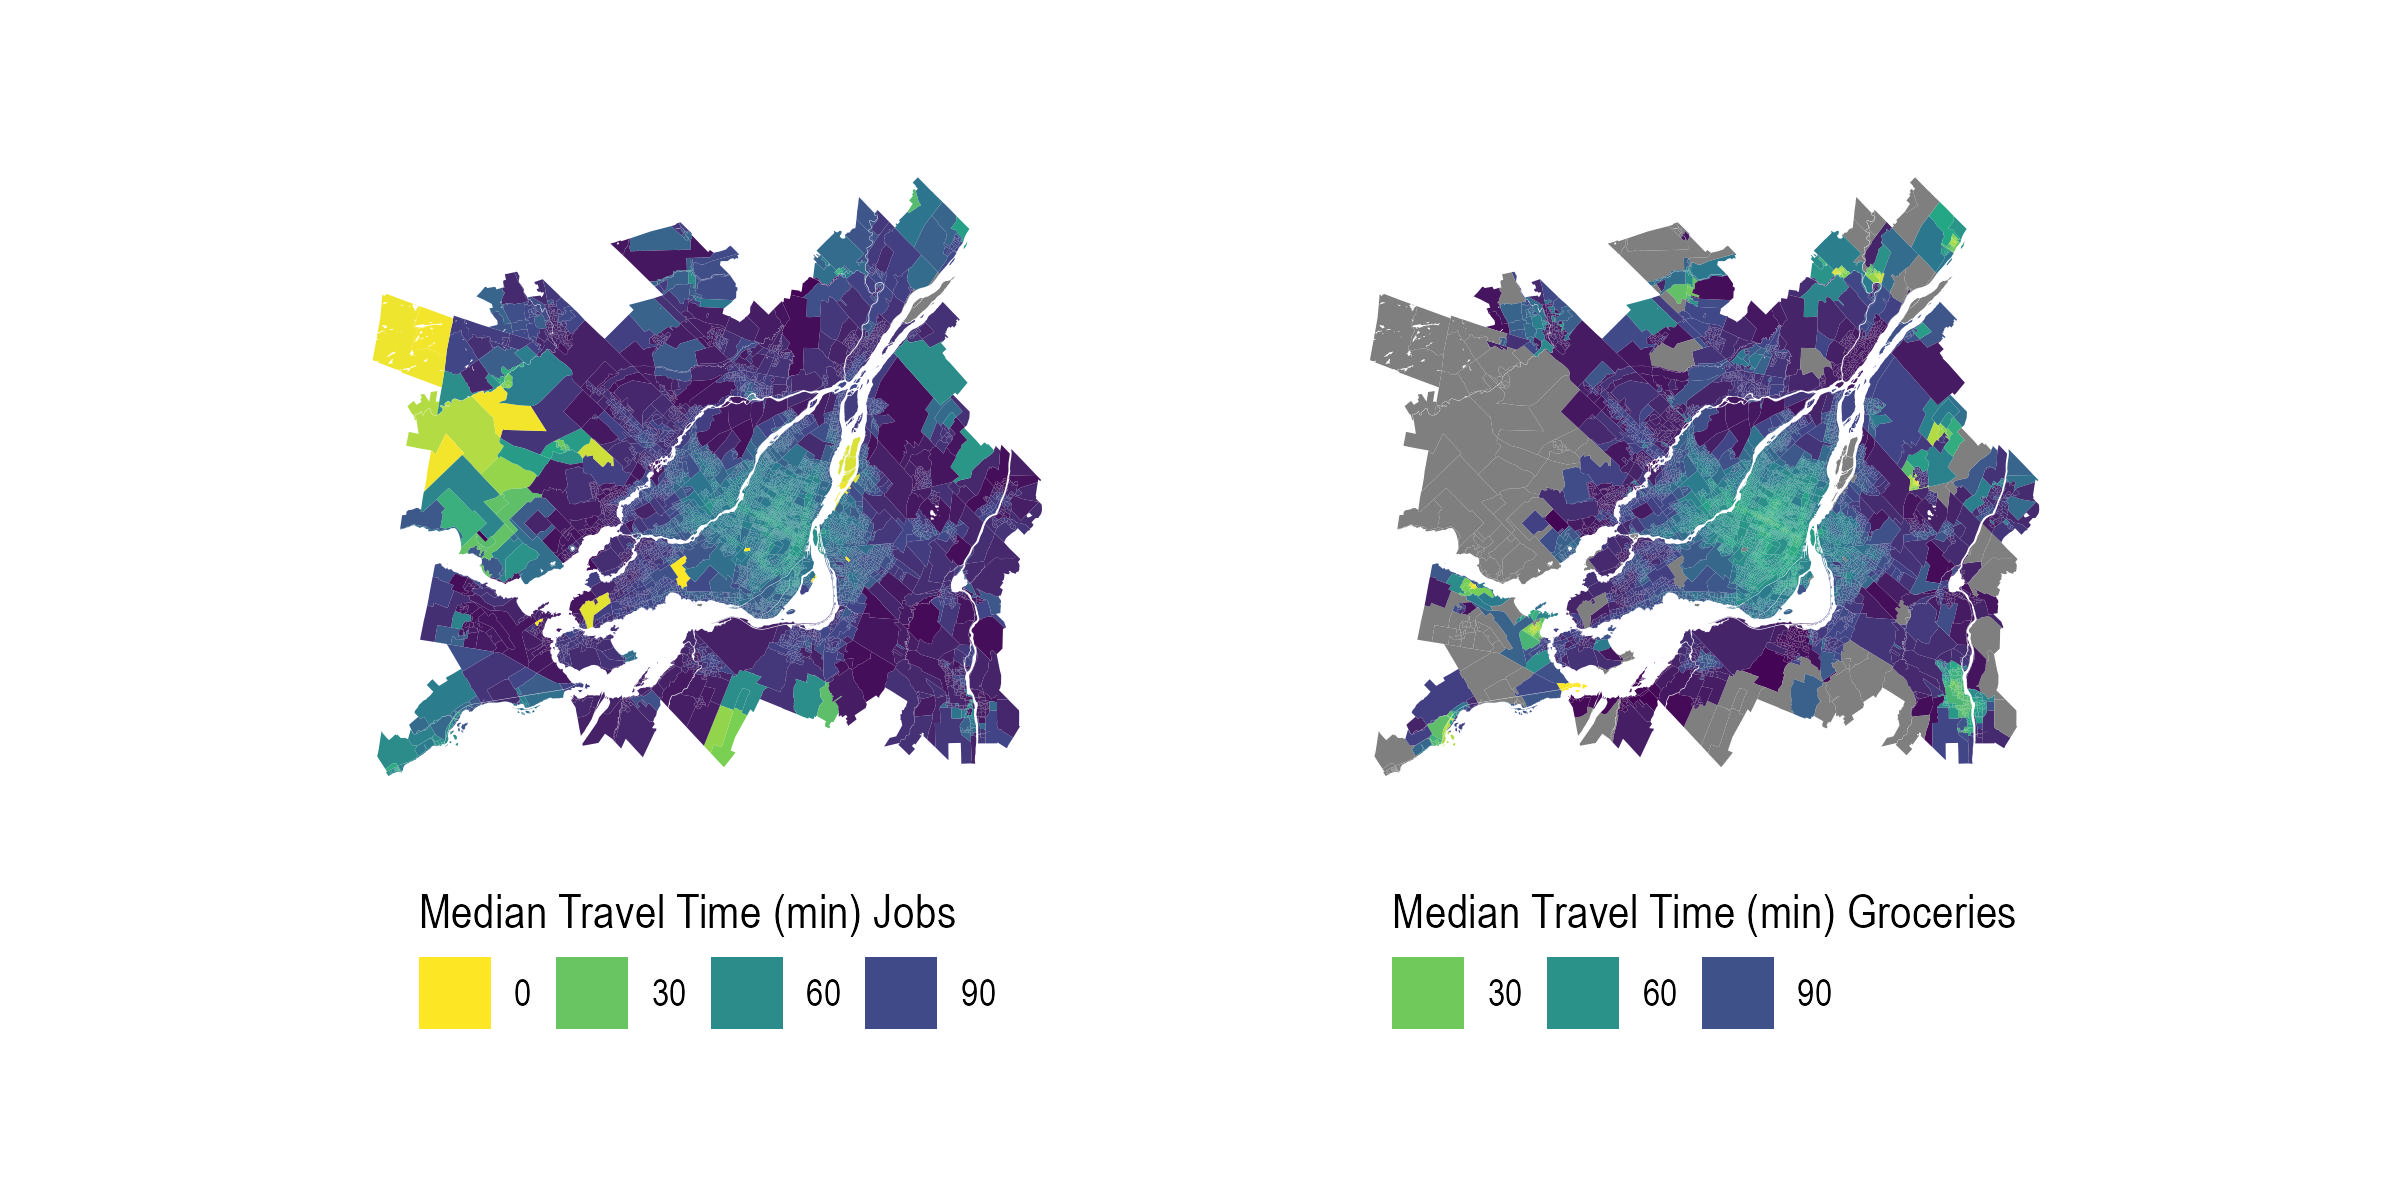
\includegraphics[width=1\linewidth]{../figures/patch_tt_emp_grc} \caption{Estimated median travel time (minutes) per Dissemination Area to jobs (left) and groceries stores (right). Public transit travel times are calculated using {r5r} (Pereira et al., 2021). DA and planning boundaries of the Montréal metropolitan area (Statistics Canada, 2016).}\label{fig:fig-travel_time_emp_grc_plot}
\end{figure}

A more thorough example of the package's use can be found on the School
of Cities' recent report on Canada's Urban Infrastructure Deficit. In
its 11th Chapter, we use the travel time matrices to estimate
accessibility metrics to jobs and groceries stores before and after the
pandemic \citep{pargaDemocraticAccessOur2024}. We then compare how
changes affected groups differently according to their spatial
distribution and income level, thus making explicit the connection of
the package's information and matters of equity in transportation. The
report is freely available for download at the State of Cities Summit
\href{https://stateofcitiessummit.ca/report}{website}.

\section{Concluding remarks}\label{concluding-remarks}

In this paper, we describe the \{canaccesR\} data package, created using
the \{r5r\} package and transit schedule, street network, employment,
and population data. The package's main contents refers to the
ready-to-use travel time matrices for public transit to reach employment
and groceries stores in Canada's 12 largest urban areas. We expect the
contents of the package to be used in transportation accessibility
evaluations within and across those regions. Moreover, these datasets
can be used in further equity assessments that evaluate the distribution
of accessibility across space and between social groups. Furthermore, in
the spirit of open data products
\citep{arribas-belOpenDataProductsA2021}, the package can be expanded
through collaboration with other researchers by, for example, including
travel time matrices to other essential destinations within the DMTI's
dataset (\emph{e.g.}, schools, healthcare, etc.). In other words, we
hope that by making these datasets publicly available, future analysis
can contribute to making Canada's transportation system more just and
fair, considering accessibility's as the main social good of
transportation \citep{martensTransportJusticeDesigning2016}, and the
inherent connection between public transit and the ``right to the city''
\citep{cogginRightTransportMoving2015}.

\section{Declaration of Conflicting
Interests}\label{declaration-of-conflicting-interests}

The author(s) declared no potential conflicts of interest with respect
to the research, authorship, and/or publication of this article.

\section{Funding}\label{funding}

The author(s) disclosed receipt of the following financial support for
the research, authorship, and/or publication of this article: This work
was supported by the Social Sciences and Humanities Research Council of
Canada (\emph{More description about the funding source after the review
process}).

\section{ORCID}\label{orcid}

\begin{itemize}
\tightlist
\item
  name: João Pedro Figueira Amorim Parga orcid: 0000-0002-4105-5927
\item
  name: Anastasia Soukhov orcid: 0000-0003-4371-4831
\item
  name: Robert Nutifafa Arku orcid: 0000-0002-2018-886X
\item
  name: Christopher Higgins orcid: 0000-0002-3551-7750
\item
  name: Antonio Páez orcid: 0000-0001-6912-9919
\end{itemize}

\section{Data availability statement}\label{data-availability-statement}

The \{canaccessR\} data package can be found and installed on its Github
\href{https://github.com/paezha/canaccessR}{respository}.

\bibliographystyle{sageh}
\bibliography{bibfile.bib}


\end{document}
